%
% This is the LaTeX template file for lecture notes for CS294-8,
% Computational Biology for Computer Scientists.  When preparing 
% LaTeX notes for this class, please use this template.
%
% To familiarize yourself with this template, the body contains
% some examples of its use.  Look them over.  Then you can
% run LaTeX on this file.  After you have LaTeXed this file then
% you can look over the result either by printing it out with
% dvips or using xdvi.
%
% This template is based on the template for Prof. Sinclair's CS 270.

\documentclass[twoside]{article}
\usepackage{graphics}
\usepackage{amsmath}
\usepackage{amssymb}
\usepackage{hyperref}
\usepackage{IEEEtrantools}
\usepackage{graphicx}

\setlength{\oddsidemargin}{0.25 in}
\setlength{\evensidemargin}{-0.25 in}
\setlength{\topmargin}{-0.6 in}
\setlength{\textwidth}{6.5 in}
\setlength{\textheight}{8.5 in}
\setlength{\headsep}{0.75 in}
\setlength{\parindent}{0 in}
\setlength{\parskip}{0.1 in}

%
% The following commands set up the lecnum (lecture number)
% counter and make various numbering schemes work relative
% to the lecture number.
%
\newcounter{lecnum}
\renewcommand{\thepage}{\thelecnum-\arabic{page}}
\renewcommand{\thesection}{\thelecnum.\arabic{section}}
\renewcommand{\theequation}{\thelecnum.\arabic{equation}}
\renewcommand{\thefigure}{\thelecnum.\arabic{figure}}
\renewcommand{\thetable}{\thelecnum.\arabic{table}}

%
% The following macro is used to generate the header.
%
\newcommand{\lecture}[4]{
   \pagestyle{myheadings}
   \thispagestyle{plain}
   \newpage
   \setcounter{lecnum}{#1}
   \setcounter{page}{1}
   \noindent
   \begin{center}
   \framebox{
      \vbox{\vspace{2mm}
    \hbox to 6.28in { {\bf CMPUT 652: Reinforcement Learning with Robots
                        \hfill Fall 2019} }
       \vspace{4mm}
       \hbox to 6.28in { {\Large \hfill Lecture #1: #2  \hfill} }
       \vspace{2mm}
       \hbox to 6.28in { {\it Instructor: #3 \hfill Scribe: #4} }
      \vspace{2mm}}
   }
   \end{center}
   \markboth{Lecture #1: #2}{Lecture #1: #2}
   {\bf Disclaimer}: {\it These notes have not been subjected to the
   usual scrutiny reserved for formal publications.  They may be distributed
   outside this class only with the permission of the Instructor.}
   \vspace*{4mm}
}

%
% Convention for citations is authors' initials followed by the year.
% For example, to cite a paper by Leighton and Maggs you would type
% \cite{LM89}, and to cite a paper by Strassen you would type \cite{S69}.
% (To avoid bibliography problems, for now we redefine the \cite command.)
% Also commands that create a suitable format for the reference list.
\renewcommand{\cite}[1]{[#1]}
\def\beginrefs{\begin{list}%
        {[\arabic{equation}]}{\usecounter{equation}
         \setlength{\leftmargin}{2.0truecm}\setlength{\labelsep}{0.4truecm}%
         \setlength{\labelwidth}{1.6truecm}}}
\def\endrefs{\end{list}}
\def\bibentry#1{\item[\hbox{[#1]}]}

%Use this command for a figure; it puts a figure in wherever you want it.
%usage: \fig{NUMBER}{SPACE-IN-INCHES}{CAPTION}
\newcommand{\fig}[3]{
			\vspace{#2}
			\begin{center}
			Figure \thelecnum.#1:~#3
			\end{center}
	}
% Use these for theorems, lemmas, proofs, etc.
\newtheorem{theorem}{Theorem}[lecnum]
\newtheorem{lemma}[theorem]{Lemma}
\newtheorem{proposition}[theorem]{Proposition}
\newtheorem{claim}[theorem]{Claim}
\newtheorem{corollary}[theorem]{Corollary}
\newtheorem{definition}[theorem]{Definition}
\newenvironment{proof}{{\bf Proof:}}{\hfill\rule{2mm}{2mm}}

% **** IF YOU WANT TO DEFINE ADDITIONAL MACROS FOR YOURSELF, PUT THEM HERE:

%%===========================================================================
%% defining the expectation operator
%%---------------------------------------------------------------------------
\DeclareMathOperator{\E}{\mathbb{E}}
%%===========================================================================

\begin{document}
%FILL IN THE RIGHT INFO.
%\lecture{**LECTURE-NUMBER**}{**DATE**}{**LECTURER**}{**SCRIBE**}
\lecture{7}{September 10}{Rupam Mahmood}{Yufeng Yuan}
%\footnotetext{These notes are partially based on those of Nigel Mansell.}

% **** YOUR NOTES GO HERE:

% Some general latex examples and examples making use of the
% macros follow.  
%**** IN GENERAL, BE BRIEF. LONG SCRIBE NOTES, NO MATTER HOW WELL WRITTEN,
%**** ARE NEVER READ BY ANYBODY.

\section{Finite Markov Decision Process}
\subsection{Formal Definition}
\subsection{Transistion Probability and Return}
\subsection{Small Example of MDP}

\begin{figure}[!hbp]
  %\centering
  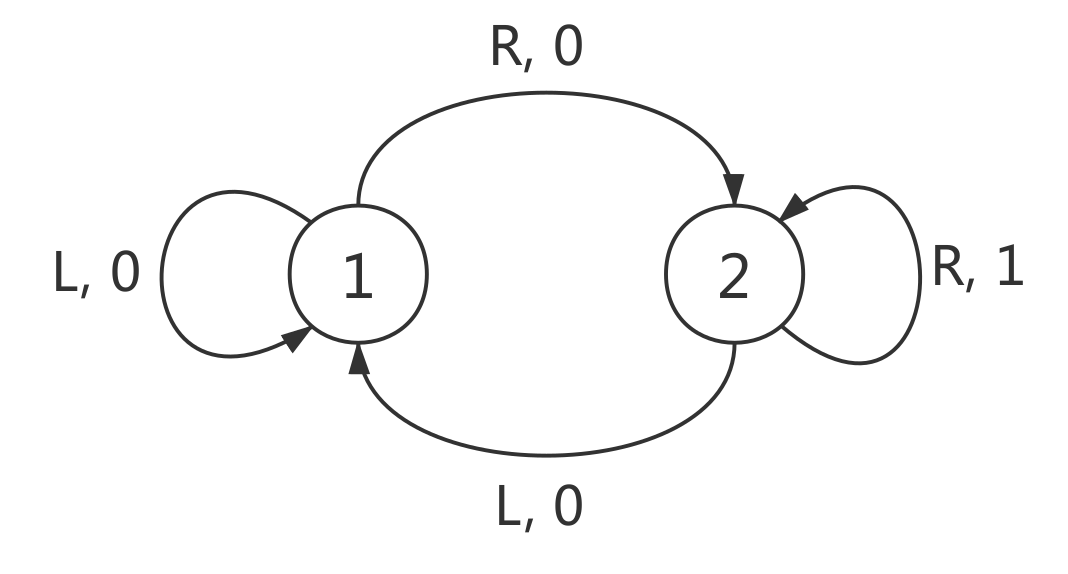
\includegraphics[scale=0.2]{images/mdp.png}
  %\caption{A learning scenario where the space of parameterized functions doesn't contain the ideal function $f^*$. In such cases, the function closest to $f^*$ is found instead.}
  \label{fig: function_space}
\end{figure}

%\centering{$\gamma=0.9$}
\begin{table}[htb!]
%\centering
\begin{tabular}{c|cccc}
\hline
$p(s', r|s,a)$ & 1,0 & 1,1 & 2,0 & 2,1 \\
\hline
$p(\cdot, \cdot|1, L)$ & 1 & 0 & 0 & 0 \\
\hline
$p(\cdot, \cdot|1, R)$ & 0 & 0 & 1 & 0 \\
\hline
$p(\cdot, \cdot|2, L)$ & 1 & 0 & 0 & 0 \\
\hline
$p(\cdot, \cdot|2, R)$ & 0 & 0 & 0 & 1 \\
\hline



\end{tabular}
\end{table}


\section{Introduction}

The use of machine learning to solve problems involves the following three broad steps:
\begin{itemize}
\item Approximating the ideal function (or the function to learn) with a parameterized function
\item Defining the learning problem in terms of an objective function
\item Deriving the learning methods from first principles
\end{itemize}

In the following sections, we will discuss each of these processes in more detail.

\subsection{Formulating a parameterized function}
A function $f$ is defined as a mapping from different inputs $X$ to their corresponding outputs $Y$. In our setting, we wish to learn an ``ideal'' function $f^*$ which is generating the data $X, Y$. Further, we wish to learn the ideal function using this data. One possible way to solve this problem is to fix a function $h = g(X)$ using human intuition.

Another approach, using Machine Learning, is to define a class or a space of functions $F_\theta = f(X; \theta)$ parameterized by some $\theta \in \Theta$. We then try to find the optimal parameter $\theta^*$ for which the difference between the ideal function $f^*$ and the parameterized function $F_{\theta^*} = f(X; \theta^*)$ is least. As illustrated in Fig. \ref{fig: function_space}, it is possible to have a case where $F_\theta$ cannot represent the ideal function; in these cases the closest match is used instead.

\begin{figure}[!hbp]
  \centering
  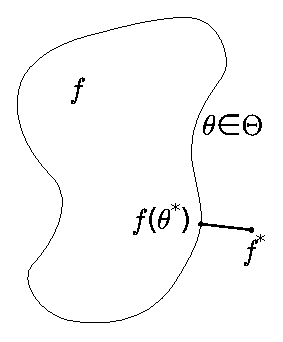
\includegraphics[scale=0.7]{images/function_space.eps}
  \caption{A learning scenario where the space of parameterized functions doesn't contain the ideal function $f^*$. In such cases, the function closest to $f^*$ is found instead.}
  \label{fig: function_space}
\end{figure}

\subsection{Defining an objective function}
After formulating a parameterized function, we need to define an objective in order to evaluate the parameterized function. The optimal parameter $\theta^*$ minimizes this objective function. There can be two types of objective functions:
\begin{enumerate}
\item Exact objective function: The complete form for an exact objective function is known, and there is no randomness associated with it. Such functions are mostly not available for real--world problems. However, they can be formulated for toy--problems and are useful for testing optimization algorithms. We represent exact objective functions as $\upsilon(\theta)$, where $\theta$ is the learnable parameter.
\item Sample--based objective function: These functions are noisy evaluations of the parameterized function based on observed data samples. We represent it as $\ell(X, F_\theta, Z)$, where $X$ is the input data, $F_\theta$ is the parameterized function, and $Z$ is the output of this parameterized function on input data. We expect the sample--based objective functions to be unbiased estimators of their corresponding exact functions: $\E[\ell(X, F_\theta, Z)] = \upsilon(\theta)$.
\end{enumerate}

\subsection{Learning Methods}
Once the objective function has been formulated, the optimal parameter $\theta^*$ is found by minimizing the objective function: $\theta^* = \arg \min_{\theta \in \Theta} \upsilon(\theta)$, or $\theta^* = \arg \min_{\theta \in \Theta} \ell(X, F_\theta, Z)$. One possible way to solve this problem is by learning the parameters incrementally:
\begin{equation}
  \theta_{t+1} = \theta_t + \Delta \theta_t, \label{eq: update_rule}
\end{equation}

where the parameter at each subsequent iteration decreases the value of the objective function. Two such incremental learning rules are Gradient descent: $\Delta \theta_t = -\alpha_t \nabla_\theta \upsilon(\theta)$ and Stochastic Gradient Descent: $\Delta \theta_t = -\alpha_t \nabla_\theta \ell(X, F_\theta, Z)$, where $\alpha_t$ is the step--size at timestep $t$ in both the cases.

\subsubsection*{Tabular Methods}
Instead of using parameterized functions to approximate the ideal function, an alternative is to use tabular representation. In this case, the function outputs a fixed value for each entry of the table and in effect has no input (so the table can be viewed as being composed of multiple functions). We represent the tabular function as $f(\theta) = \theta$. The ideal function in this case would be $f^*$ (basically a constant) and we try to find $\theta^*$ such that $f(\theta^*)$ is closest to $f^*$.

\section{Deriving squared loss from Maximum Likelihood Estimate}
Consider a situation where we observe data sampled from a Normal distribution, with our goal being to estimate the mean of this Normal distribution using the observed data. Assume we observe the random variable $Y \sim \mathcal{N}(\theta^*, \sigma)$, with $\theta^*$ being the true mean of the underlying Normal distribution and $\sigma$ its standard deviation.

In using Maximum Likelihood Estimate, we try to maximize the log probability of drawing the observation given the mean $\theta$. That is
\begin{IEEEeqnarray}{lCl}
  \theta^* &=& \arg \max_{\theta \in \Theta} \; \log p(\{Y_i\}_{i=1}^N \;|\; \theta) \\
  &=& \arg \max_{\theta \in \Theta} \; \log \prod_{i=1}^N \frac{1}{\sqrt{2 \pi \sigma^2}} e^{-\frac{(Y_i - \theta)^2}{2 \sigma^2}} \nonumber \\
  &=& \arg \max_{\theta \in \Theta} \; \left[ -\frac{N}{2} \log (2 \pi \sigma^2) - \sum_{i=1}^N \frac{(Y_i - \theta)^2}{2 \sigma^2} \right] \nonumber \\
  &=& \arg \min_{\theta \in \Theta} \; \sum_{i=1}^N (Y_i - \theta)^2,
\end{IEEEeqnarray}

which is the sample--based batched loss function $\ell(F_\theta, \{Y_i\}_{i=1}^t) = \sum_{i=1}^N (Y_i - \theta)^2$.

We can use this loss function to calculate the exact form for the stochastic gradient descent update: $\Delta \theta_t = - \alpha \nabla_\theta \ell(F_\theta, Y_t) = 2 \alpha_t (Y_t-\theta)$. The resulting update equation is
\begin{equation}
  \theta_{t+1} = \theta_t + 2 \alpha_t (Y_t - \theta_t). \label{eq: sgd_update}
\end{equation}

\subsection{Method of Averages}
Our problem is to obtain the optimal parameter $\tilde{\theta}_{t+1}$ which minimizes the loss function $\ell(F_\theta, \{Y_i\}_{i=1}^t) = \sum_{i=1}^N (Y_i - \theta)^2$; i.e. $\tilde{\theta}_{t+1} = \arg \min_{\theta \in \Theta} \ell(F_\theta, \{Y_i\}_{i=1}^t)$. Instead of using the incremental stochastic gradient descent update, we can directly obtain the optimal parameter $\tilde{\theta}_{t+1}$ by using the complete batch of data. To do so, we set the derivative of the loss with respect to $\theta$ as zero and then solve for the optimal $\theta$.
\begin{IEEEeqnarray}{lrCl}
  \quad & \frac{\partial}{\partial \tilde{\theta}_{t+1}} \sum_{i=1}^t (Y_i - \tilde{\theta}_{t+1})^2 &=& 0 \nonumber \\
  \text{or} \quad & \sum_{i=1}^t 2 (Y_i - \tilde{\theta}_{t+1}) (-1) &=& 0 \nonumber \\
  \text{or} \quad & \tilde{\theta}_{t+1} &=& \frac{1}{t} \sum_{i=1}^t Y_i. \label{eq: sample_avg}
\end{IEEEeqnarray}

From this equation, we can see that the optimal parameter which minimizes the batched least squares error is the sample average of that batch. It is possible to compute this sample average in an incremental fashion too:
\begin{equation}
  \tilde{\theta}_{t+1} = \tilde{\theta}_t + \frac{1}{t} (Y_t - \tilde{\theta}_t). \label{eq: sample_avg_incremental}
  \end{equation}

Yet another incremental form to compute the sample average is to maintain the sums for the numerator and denominator separately: $\tilde{\theta}_{t+1} = \frac{N_{t+1}}{D_{t+1}}$, with $N_{t+1} = N_t + Y_t$ and $D_{t+1} = D_t + 1$. All the three methods presented above for calculating the sample average would have different numerical stabilities. Further, note that Eq. \ref{eq: sample_avg_incremental} can be obtained from the stochastic gradient descent update (Eq. \ref{eq: sgd_update}) by putting $\alpha_t = \frac{1}{2t}$.


\subsubsection{Constant step--size update}
Another form of update uses a constant--step size $\alpha_t = \frac{\alpha}{2}$ in Eq. \ref{eq: sgd_update}, which leads to an exponentially weighted sample average:
\begin{IEEEeqnarray}{lCl}
  \theta_{t+1} &=& \theta_t + \alpha (Y_t - \theta_t) \nonumber \\
  &=& (1 - \alpha) \theta_t  + \alpha Y_t \nonumber \\
  &\vdots& \nonumber \\
  &=& (1-\alpha)^{t+1} \theta_0 + \alpha (1 - \alpha)^t Y_0  + \cdots + \alpha (1 - \alpha) Y_{t-1} + \alpha Y_t \nonumber \\
  &=& (1-\alpha)^{t+1} \theta_0 + \sum_{i=0}^t \alpha (1-\alpha)^{t-i} Y_i. \label{eq: constant_step_size_estimate}
\end{IEEEeqnarray}

\section{Bias and Variance of different estimates}
We first show the bias--variance decomposition of the exact objective function, in this case the Mean Squared Error (MSE), and then proceed to calculate the bias and variance of the sample average method and the exponential average method.
\begin{IEEEeqnarray}{lCl}
  \upsilon(\tilde{\theta}_{t+1})
  &=& \E[(Y - \tilde{\theta}_{t+1})^2] \\
  &=& \E[(\theta^* - \tilde{\theta}_{t+1} + Y - \theta^*)^2] \\
  &=& \E[(\theta^* - \tilde{\theta}_{t+1})^2 + (Y - \theta^*)^2 + 2(\theta^* - \tilde{\theta}_{t+1})(Y - \theta^*)] \\
  &=& \E[(\theta^* - \tilde{\theta}_{t+1})^2] + \underbrace{\E[(Y - E[Y])^2]}_{\text{Variance of outcome}} + \underbrace{\E[2(\theta^* - \tilde{\theta}_{t+1})(Y - \theta^*)]}_{0} \\
  &=& \E[(\theta^* - \E[\tilde{\theta}_{t+1}] + \E[\tilde{\theta}_{t+1}] - \tilde{\theta}_{t+1})^2] + \text{Var}(Y) \nonumber \\
  &=& \E[(\theta^* - \E[\tilde{\theta}_{t+1}])^2] + \underbrace{\E[(\E[\tilde{\theta}_{t+1}] - \tilde{\theta}_{t+1})^2]}_{\text{Variance of estimate}} + 2 \underbrace{\E[(\theta^* - \E[\tilde{\theta}_{t+1}])(\E[\tilde{\theta}_{t+1}] - \tilde{\theta}_{t+1})]}_{0} + \text{Var}(Y) \nonumber \\
  &=& \underbrace{(\theta^* - \E[\tilde{\theta}_{t+1}])^2}_{\text{Bias}^2} + \text{Var}(\tilde{\theta}_{t+1}) + \text{Var}(Y).
\end{IEEEeqnarray}

\subsection{Bias and Variance of Sample Average Method}
We now calculate the bias of the sample average estimate:
\begin{IEEEeqnarray}{lCl}
  \text{Bias}(\tilde{\theta}_{t+1}) &=& \E[\tilde{\theta}_{t+1}] - \theta^* \nonumber \\
  &=& \E\left[\frac{1}{t} \sum_{i=1}^t Y_i\right] - \theta^* \nonumber \\
  &=& \frac{1}{t} \cdot t \E[Y] - \theta^* \nonumber \\
  &=& \theta^* - \theta^* \nonumber \\
  &=& 0,
\end{IEEEeqnarray}

where in the second line we replaced $\tilde{\theta}_{t+1}$ with the sample average from Eq. \ref{eq: sample_avg} and in the fourth line we replaced $\E[Y]$ with $\theta^*$ since $Y \sim \mathcal{N}(\theta^*, \sigma)$. From this equation, we see that the sample average is an unbiased estimator of the true sample mean.

The variance of the sample average estimate is:
\begin{IEEEeqnarray}{lCl}
  \text{Var}(\tilde{\theta}_{t+1}) &=& \E[\tilde{\theta}_{t+1}^2] - \E[\tilde{\theta}_{t+1}]^2 \nonumber \\
  &=& \E\left[\left(\frac{1}{t} \sum_{i=1}^t Y_i\right)^2\right] - {\theta^*}^2 \nonumber \\
  &=& \frac{1}{t^2} \E \left[ \sum_{i=1}^t Y_i^2 + \mathop{\sum_{i=1}^t\sum_{j=1}^t}_{i \neq j} Y_i Y_j \right] - {\theta^*}^2 \nonumber \\
  &=& \frac{1}{t^2} \sum_{i=1}^t \E[Y_i^2] + \frac{1}{t^2} \mathop{\sum_{i=1}^t \sum_{j=1}^t}_{i \neq j} \E[Y_i] \E[Y_j] - {\theta^*}^2 \nonumber \\
  &=& \frac{1}{t^2} \cdot t ({\theta^*}^2 + \sigma^2) + \frac{t(t-1)}{t^2} {\theta^*}^2 - {\theta^*}^2 \nonumber \\
  &=& \frac{\sigma^2}{t},
\end{IEEEeqnarray}

where in the second line we used the result obtained in the previous paragraph that $\E[\tilde{\theta}_{t+1}] = {\theta^*}$, in the fourth line we split the expectation operator over the product $Y_i Y_j$ because both of them are sampled i.i.d. from a normal distribution, and in the fifth line we replaced $\E[Y_i^2]$ with $({\theta^*}^2 + \sigma^2)$ using the definition of variance. We observe that the variance of the sample average asymptotically goes to zero as the number of samples used to calculate the average increase.

\subsection{Bias and Variance of Constant Step--size Estimate}
The constant step--size estimate is $\theta_{t+1} = (1-\alpha)^{t+1} \theta_0 + \sum_{i=0}^t \alpha (1-\alpha)^{t-i} Y_i$ from Eq. \ref{eq: constant_step_size_estimate}. We now calculate the bias of this estimate:
\begin{IEEEeqnarray}{lCl}
  \text{Bias}(\theta_{t+1}) &=& \E[\theta_{t+1}] - \theta^* \nonumber \\
  &=& \E\left[(1-\alpha)^{t+1} \theta_0 + \sum_{i=0}^t \alpha (1-\alpha)^{t-i} Y_i\right] - \theta^* \nonumber \\
  &=& (1-\alpha)^{t+1} \theta_0 + \sum_{i=0}^t \alpha (1-\alpha)^{t-i} \E[Y_i] - \theta^* \nonumber \\
  &=& (1-\alpha)^{t+1} \theta_0 + \alpha \theta^* \sum_{i=0}^t (1-\alpha)^{t-i} - \theta^* \nonumber \\
  &=& (1-\alpha)^{t+1} \theta_0 + \alpha \theta^* \frac{1-(1-\alpha)^{t+1}}{1-(1-\alpha)} - \theta^* \nonumber \\
  &=& (1-\alpha)^{t+1} (\theta_0 - \theta^*).
\end{IEEEeqnarray}

If we assume that $-1<1-\alpha<1$, that is, $0 < \alpha < 2$, then we see that the bias of the constant--step size estimate asymptotically goes to zero as the number of samples observed increases.

The variance calculation is:
\begin{IEEEeqnarray}{lCl}
  \text{Var}(\theta_{t+1}) &=& \text{Var}\left( (1-\alpha)^{t+1} \theta_0 + \sum_{i=0}^t \alpha (1-\alpha)^{t-i} Y_i \right) \nonumber \\
  &=& \text{Var}((1-\alpha)^{t+1} \theta_0) + \sum_{i=0}^t (\alpha (1-\alpha)^{t-i})^2 \; \text{Var}(Y_i)) \nonumber \\
  &=& 0 + \sigma^2 \alpha^2 \sum_{i=0}^t (1-\alpha)^{2(t-i)} \nonumber \\
  &=& \sigma^2 \alpha^2 \frac{1 - (1-\alpha)^{2(t+1)}}{1 - (1-\alpha)^2} \nonumber \\
  &=& \alpha \frac{1 - (1-\alpha)^{2(t+1)}}{2 - \alpha} \sigma^2,
\end{IEEEeqnarray}

where because of the fact that $\theta_0$ and all the $Y_i\text{s}$ are independent of each other, we use the rules $\text{Var}(X + Y) = \text{Var}(X) + \text{Var}(Y)$, $\text{Var}(aX) = a^2 \text{Var}(X)$, and $\text{Var}(a) = 0$ with $X$ and $Y$ being independent random variables and $a$ a constant. Again if we assume that $0 < \alpha < 2$, the $\text{Var}(\theta_{t+1})$ asymptotically goes to $\frac{\alpha}{2 - \alpha} \sigma^2$ as the value of $t$ increases.

%% Verification of the above Variance calculation by the definition of variance
%% \begin{IEEEeqnarray*}{lCl}
%%   \text{Var}(\theta_{t+1}) &=& \E[\theta_{t+1}^2] - \E[\theta_{t+1}]^2 \\
%%   &=& \E\left[\left( (1-\alpha)^{t+1} \theta_0 + \sum_{i=0}^t \alpha (1-\alpha)^{t-i} Y_i \right)^2\right] - \left((1-\alpha)^{t+1} (\theta_0 - \theta^*) + \theta^*\right)^2 \\
%%   &=& (1-\alpha)^{2(t+1)} \theta_0^2 + \alpha^2 \sum_{i=0}^t (1-\alpha)^{2(t-i)} \E[Y_i^2] + \alpha^2 \mathop{\sum_{i=1}^t\sum_{j=1}^t}_{i \neq j} (1-\alpha)^{2t-i-j}  \E\left[Y_i Y_j\right] \\
%%   && \qquad + 2 \alpha (1-\alpha)^{t+1} \theta_0 \sum_{i=0}^t (1-\alpha)^{t-i} \E[Y_i] - \left((1-\alpha)^{t+1} (\theta_0 - \theta^*) + \theta^*\right)^2 \\
%%   &=& (1-\alpha)^{2(t+1)} \theta_0^2 + \alpha^2 ({\theta^*}^2 + \sigma^2) \sum_{i=0}^t (1-\alpha)^{2(t-i)} + \alpha^2 {\theta^*}^2 \mathop{\sum_{i=1}^t\sum_{j=1}^t}_{i \neq j} (1-\alpha)^{2t-i-j} \\
%%   && \qquad + 2 \alpha (1-\alpha)^{t+1} \theta_0 \theta^*\sum_{i=0}^t (1-\alpha)^{t-i} - \left((1-\alpha)^{t+1} (\theta_0 - \theta^*) + \theta^*\right)^2 \\
%%   &=& (1-\alpha)^{2(t+1)} \theta_0^2 + \alpha^2 \sigma^2 \sum_{i=0}^t (1-\alpha)^{2(t-i)} + \alpha^2 {\theta^*}^2 \left(\sum_{i=0}^t (1-\alpha)^{2(t-i)} + \mathop{\sum_{i=1}^t\sum_{j=1}^t}_{i \neq j} (1-\alpha)^{2t-i-j} \right) \\
%%   && \qquad + 2 \alpha (1-\alpha)^{t+1} \theta_0 \theta^*\sum_{i=0}^t (1-\alpha)^{t-i} - \left((1-\alpha)^{t+1} (\theta_0 - \theta^*) + \theta^*\right)^2 \\
%%   &=& (1-\alpha)^{2(t+1)} \theta_0^2 + \alpha^2 \sigma^2 \sum_{i=0}^t (1-\alpha)^{2(t-i)} + \alpha^2 {\theta^*}^2 \left(\sum_{i=0}^t (1-\alpha)^{t-i}\right)^2 \\
%%   && \qquad + 2 \alpha (1-\alpha)^{t+1} \theta_0 \theta^*\sum_{i=0}^t (1-\alpha)^{t-i} - \left((1-\alpha)^{t+1} (\theta_0 - \theta^*) + \theta^*\right)^2 \\
%%   &=& (1-\alpha)^{2(t+1)} \theta_0^2 + \alpha^2 \sigma^2 \frac{1 - (1-\alpha)^{2(t+1)}}{1 - (1-\alpha)^2} + \alpha^2 {\theta^*}^2 \left(\frac{1 - (1 - \alpha)^{t+1}}{1 - (1-\alpha)}\right)^2 \\
%%   && \qquad + 2 \alpha (1-\alpha)^{t+1} \theta_0 \theta^* \frac{1 - (1 - \alpha)^{t+1}}{1 - (1-\alpha)} - \left((1-\alpha)^{t+1} (\theta_0 - \theta^*) + \theta^*\right)^2 \\
%%   &=& (1-\alpha)^{2(t+1)} \theta_0^2 + \alpha \frac{1 - (1-\alpha)^{2(t+1)}}{2 - \alpha} \sigma^2 + {\theta^*}^2 \left(1 - (1 - \alpha)^{t+1}\right)^2 \\
%%   && \qquad + 2 (1-\alpha)^{t+1} \theta_0 \theta^* (1 - (1 - \alpha)^{t+1}) - \left((1-\alpha)^{t+1} (\theta_0 - \theta^*) + \theta^*\right)^2 \\
%%   &=& (1-\alpha)^{2(t+1)} \theta_0^2 + {\theta^*}^2 (1 - \alpha)^{2(t+1)} + {\theta^*}^2 - 2 {\theta^*}^2 (1 - \alpha)^{t+1} - 2 (1-\alpha)^{2(t+1)} \theta_0 \theta^* \\
%%   && \qquad + 2 (1-\alpha)^{t+1} \theta_0 \theta^* - \left((1-\alpha)^{t+1} (\theta_0 - \theta^*) + \theta^*\right)^2 + \alpha \frac{1 - (1-\alpha)^{2(t+1)}}{2 - \alpha} \sigma^2 \\
%%   &=& (1-\alpha)^{2(t+1)} (\theta_0 - \theta^*)^2 + {\theta^*}^2 + 2 \theta^* (1 - \alpha)^{t+1} (\theta_0 - \theta^*) - \left((1-\alpha)^{t+1} (\theta_0 - \theta^*) + \theta^*\right)^2 \\
%%   && \qquad + \alpha \frac{1 - (1-\alpha)^{2(t+1)}}{2 - \alpha} \sigma^2 \\
%%   &=& \alpha \frac{1 - (1-\alpha)^{2(t+1)}}{2 - \alpha} \sigma^2.
%% \end{IEEEeqnarray*}


%% \section*{References}
%% \beginrefs
%% \bibentry{AGM97}{\sc N.~Alon}, {\sc Z.~Galil} and {\sc O.~Margalit},
%% On the Exponent of the All Pairs Shortest Path Problem,
%% {\it Journal of Computer and System Sciences\/}~{\bf 54} (1997),
%% pp.~255--262.

%% \bibentry{F76}{\sc M. L. ~Fredman}, New Bounds on the Complexity of the 
%% Shortest Path Problem, {\it SIAM Journal on Computing\/}~{\bf 5} (1976), 
%% pp.~83-89.
%% \endrefs


\end{document}





